
\section{Introduction}
\label{sec:introduction}
%%% General intro
\IEEEPARstart{T}{he} constant research and the rapid evolution of artificial neural networks (ANNs) are driving the transition to smarter and more powerful AI applications, where CNN-based models represent the essential building blocks of deep learning algorithms in computer vision tasks \cite{hassaballah2020deep}. Applications such as smart surveillance, medical imaging, natural language processing, robotics, and autonomous navigation have been powered by CNN-based models in industry and academia \cite{dhillon2020convolutional}. Nonetheless, dedicated hardware is often required to accelerate execution due to the high computational demands of CNNs. In terms of pure computational throughput, graphics processing units (GPUs) offer the best performance. In terms of power consumption, FPGA solutions are well known to be more energy efficient (than GPUs) \cite{nurvitadhi2017can}. As a result, numerous FPGA accelerators have been proposed, targeting both high performance computing (HPC) for data-centers and embedded systems applications \cite{abdelouahab2018accelerating, moini2017resource, guo2017angel}. However, most commercial deep learning processing units (DPUs) are not designed for low-power, resource-limited embedded FPGAs.

In this paper, we present a tensor processor compatible with TensorFlow Lite to accelerate \emph{Conv2D} and \emph{DepthwiseConv2D} operations on embedded FPGA. This implementation is integrated in a hardware/software co-design framework to accelerate tensor operations on FPGAs. This framework integrates TensorFlow Lite library and implements delegate interfaces\cite{TensorFlowDelegate} as bridge between the TF Lite runtime and the proposed hardware architecture. To control resource utilization and energy consumption, we implement the tensor operations as individual hardware engines, where they are optionally instantiated in the FPGA fabric as needed. Further on, to accelerate floating-point computation, we adopt the hybrid custom floating-point and logarithmic dot-product approximation technique\cite{nevarez2021accelerating}, which exploits the intrinsic error-resilience of neural networks \cite{venkataramani2015approximate}. This approach can efficiently trade off quality-of-result (QoR) and resource utilization.

\begin{figure}[t!]
	\centering
	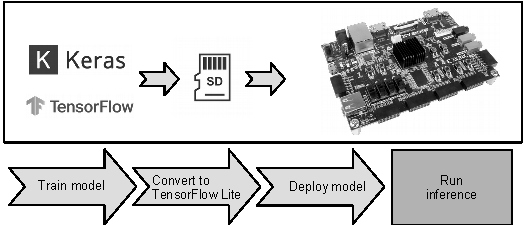
\includegraphics[width=0.5\textwidth]{../figures/workflow.pdf}
	\caption{Deployment workflow.}
	\label{fig:workflow}
\end{figure}

To operate the proposed system, the user would train a custom CNN model using TensorFlow or Keras, then this is converted into a TensorFlow Lite model, then the model is stored in a micro SD card along with the embedded software and configuration bitstream. See \Fig{fig:workflow}.

Our main contributions are as follows:
\begin{enumerate}
	\item We present a tensor processor as a dedicated hardware accelerator for TensorFlow Lite on embedded FPGA. We accelerate \emph{Conv2D} and \emph{DepthwiseConv2D} tensor operations with fixed-point and floating-point computation.
	\item We develop a hardware/software co-design framework targeting low-power and resource-constrained AI applications. The parameterized and modular architecture enables design exploration with different compute hardware approaches.
	\item We demonstrate the potential of the proposed architecture by address a design exploration of \emph{Conv2D} and \emph{DepthwiseConv2D} operations with four compute engines: (1) fixed-point, (2) floating-point LogiCORE, (3) hybrid custom floating-point approximation, and (4) hybrid logarithmic approximation. We evaluate compute performance and classification accuracy implementing half-precision, brain floating-point, TensorFloat, and custom reduced formats for approximate processing, including logarithmic computation. Detailed performance reports are presented.
\end{enumerate}

To promote the research in this field, our entire work is made available to the public as an open-source project at X.